\documentclass[tikz,border=2mm]{standalone}
\usepackage{amsmath,amssymb}
\usepackage{xcolor}
\usepackage{pifont}
\usetikzlibrary{positioning,arrows.meta,shapes.geometric,shadows.blur,decorations.pathreplacing,calc,fit,backgrounds}

\definecolor{jbrand}{RGB}{15,58,102}
\definecolor{jbrandlight}{RGB}{232,240,247}
\definecolor{jbrandline}{RGB}{184,206,224}
\definecolor{jgrey}{RGB}{90,90,90}
\definecolor{jamber}{RGB}{176,98,10}
\definecolor{jamberlight}{RGB}{250,240,224}

\begin{document}
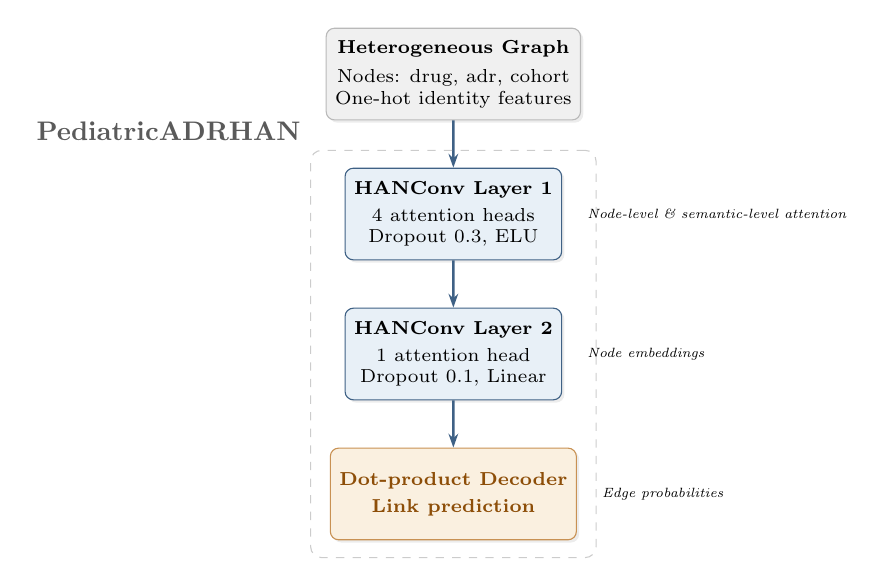
\begin{tikzpicture}[
  scale=0.97, every node/.append style={scale=0.97},
  font=\scriptsize,
  pipebox/.style={rectangle,rounded corners=3pt,draw=jbrand!80,fill=jbrandlight,
    minimum width=2cm,minimum height=1.2cm,align=center,
    drop shadow={shadow xshift=1pt,shadow yshift=-1pt,opacity=0.15}},
  layerbox/.style={pipebox,fill=gray!12,draw=gray!55},
  gatebox/.style={pipebox,fill=jamberlight,draw=jamber!70,font=\scriptsize\bfseries,text=jamber!80!black},
  arr/.style={-{Stealth[length=5pt,width=3.5pt]},line width=0.9pt,color=jbrand!80},
]

\node[layerbox, align=center] (INPUT) at (0,0) {\textbf{Heterogeneous Graph}\\[3pt]Nodes: drug, adr, cohort\\One-hot identity features};
\node[pipebox, below=0.6cm of INPUT] (L1) {\textbf{HANConv Layer 1}\\[2pt]4 attention heads\\Dropout 0.3, ELU};
\node[pipebox, below=0.6cm of L1] (L2) {\textbf{HANConv Layer 2}\\[2pt]1 attention head\\Dropout 0.1, Linear};
\node[gatebox, below=0.6cm of L2] (DEC) {\textbf{Dot-product Decoder}\\[2pt]Link prediction};

\draw[arr] (INPUT) -- (L1);
\draw[arr] (L1) -- (L2);
\draw[arr] (L2) -- (DEC);

\node[font=\tiny\itshape,right=0.2cm of L1] {Node-level \& semantic-level attention};
\node[font=\tiny\itshape,right=0.2cm of L2] {Node embeddings};
\node[font=\tiny\itshape,right=0.2cm of DEC] {Edge probabilities};

\node[rectangle, draw=gray!40, dashed, rounded corners, fit=(L1) (L2) (DEC), inner sep=0.3cm] (MODEL) {};
\node[above left, font=\bfseries\color{jgrey}] at (MODEL.north west) {PediatricADRHAN};

\end{tikzpicture}
\end{document}
